\documentclass{standalone}

\usepackage{tikz}
\usepackage{bm}
\usepackage{pgfplots}
\usetikzlibrary{calc, tikzmark, shapes, shapes.arrows, arrows, 3d, positioning}
\pgfplotsset{compat=1.17}
\begin{document}
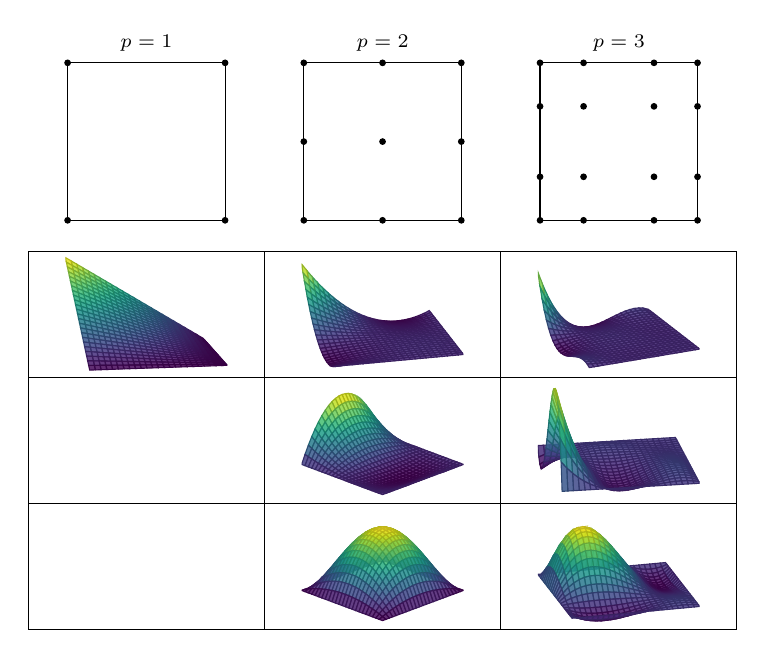
\begin{tikzpicture}
	\scriptsize
	\draw (0,0) rectangle (2,2); 
	\foreach \i in {0,2}{
		\foreach \j in {0,2}{
			\filldraw[black] (\i,\j) circle[radius=1pt]; 		
		}
	}
	\node at (1,2.25) {$p=1$}; 

	\begin{scope}[xshift=3cm]
		\draw (0,0) rectangle (2,2); 
		\foreach \i in {0,1,2}{
			\foreach \j in {0,1,2}{
				\filldraw[black] (\i,\j) circle[radius=1pt]; 		
			}
		}
		\node at (1,2.25) {$p=2$}; 
	\end{scope}

	\begin{scope}[xshift=6cm]
		\draw (0,0) rectangle (2,2); 
		\foreach \i in {0,5.52786405e-01,1.44721360e+00,2}{
			\foreach \j in {0,5.52786405e-01,1.44721360e+00,2}{
				\filldraw[black] (\i,\j) circle[radius=1pt]; 		
			}
		}
		\node at (1,2.25) {$p=3$}; 
	\end{scope}

	% linear shapes 
	\begin{axis}[anchor=origin, axis lines=none, colormap/viridis, view={-10}{15}, 
		scale=.3, yshift=-1.7cm, xshift=1cm]
		\addplot3[domain=-1:1, y domain=-1:1, fill opacity=.85, surf]({x},{y},{.25*(1-\x)*(1+\y)}); 
	\end{axis}

	% quadratic shapes 
	\begin{axis}[anchor=origin, axis lines=none, colormap/viridis, view={-15}{30}, 
		scale=.3, yshift=-1.5cm, xshift=4cm]
		\addplot3[domain=-1:1, y domain=-1:1, fill opacity=.85, surf]({x},{y},{(.5*\x*\x-.5*\x)*(.5*\y*\y+.5*\y)}); 
	\end{axis}
	\begin{axis}[anchor=origin, axis lines=none, colormap/viridis, view={45}{30}, 
		scale=.3, yshift=-3.1cm, xshift=4cm]
		\addplot3[domain=-1:1, y domain=-1:1, fill opacity=.85, surf]({x},{y},{(.5*\x*\x-.5*\x)*(1-\y*\y)}); 
	\end{axis}	
	\begin{axis}[anchor=origin, axis lines=none, colormap/viridis, view={45}{30}, 
		scale=.3, yshift=-4.7cm, xshift=4cm]
		\addplot3[domain=-1:1, y domain=-1:1, fill opacity=.85, surf]({x},{y},{(1-\x*\x)*(1-\y*\y)}); 
	\end{axis}

	% cubic shapes 
	\begin{axis}[anchor=origin, axis lines=none, colormap/viridis, view={-25}{30}, 
		scale=.3, yshift=-1.5cm, xshift=7cm]
		\addplot3[domain=-1:1, y domain=-1:1, fill opacity=.85, surf]({x},{y},{(-.625*\x^3+.625*\x^2+.125*\x-.125)*(.625*\y^3+.625*\y^2-.125*\y-.125)}); 
	\end{axis}
	\begin{axis}[anchor=origin, axis lines=none, colormap/viridis, view={-10}{30}, zmax=1.25,
		scale=.3, yshift=-3.1cm, xshift=7cm]
		\addplot3[domain=-1:1, y domain=-1:1, fill opacity=.85, surf]({x},{y},{2*(1.39754249*\y*\y*\y-0.625*\y*\y-1.39754249*\y+0.625)*(-0.625*\x*\x*\x+0.625*\x*\x+0.125*\x-0.125)}); 
	\end{axis}	
	\begin{axis}[anchor=origin, axis lines=none, colormap/viridis, view={-15}{30}, 
		scale=.3, yshift=-4.7cm, xshift=7cm]
		\addplot3[domain=-1:1, y domain=-1:1, fill opacity=.85, surf]({x},{y},{(1.3974*\x^3-.625*\x^2-1.3975*\x+.625)*(-1.3974*\y^3-.625*\y^2+1.3975*\y+.625)}); 
	\end{axis}	

	% bounding box 
	\begin{scope}[xshift=0, yshift=-.4cm]
		\foreach \i in {0,-1.6,-3.2,-4.8}{
			\draw (-.5,\i) -- (8.5,\i); 
		}
		\foreach \i in {-.5,2.5,5.5,8.5}{
			\draw (\i,0) -- (\i,-4.8); 
		}
	\end{scope}

\end{tikzpicture}
\end{document}